
% Author: Stefan Helmert
% used components:
%   Author: Tom Bombadil (arrows)
%   Author: Tomasz M. Trzeciak (earth)

\documentclass[tikz,border=10pt]{standalone}
\usetikzlibrary{decorations.text}
\usepackage{arrayjobx}
\usepackage{pgfmath}

%% helper macros

\newcommand\pgfmathsinandcos[3]{%
	\pgfmathsetmacro#1{sin(#3)}%
	\pgfmathsetmacro#2{cos(#3)}%
}
\newcommand\LongitudePlane[3][current plane]{%
	\pgfmathsinandcos\sinEl\cosEl{#2} % elevation
	\pgfmathsinandcos\sint\cost{#3} % azimuth
	\tikzset{#1/.style={cm={\cost,\sint*\sinEl,0,\cosEl,(0,0)}}}
}
\newcommand\LatitudePlane[3][current plane]{%
	\pgfmathsinandcos\sinEl\cosEl{#2} % elevation
	\pgfmathsinandcos\sint\cost{#3} % latitude
	\pgfmathsetmacro\yshift{\cosEl*\sint}
	\tikzset{#1/.style={cm={\cost,0,0,\cost*\sinEl,(0,\yshift)}}} %
}
\newcommand\DrawLongitudeCircle[2][1]{
	\LongitudePlane{\angEl}{#2}
	\tikzset{current plane/.prefix style={scale=#1}}
	% angle of "visibility"
	\pgfmathsetmacro\angVis{atan(sin(#2)*cos(\angEl)/sin(\angEl))} %
	\draw[current plane] (\angVis:1) arc (\angVis:\angVis+180:1);
	
}
\newcommand\DrawLatitudeCircle[2][1]{
	\LatitudePlane{\angEl}{#2}
	\tikzset{current plane/.prefix style={scale=#1}}
	\pgfmathsetmacro\sinVis{sin(#2)/cos(#2)*sin(\angEl)/cos(\angEl)}
	% angle of "visibility"
	\pgfmathsetmacro\angVis{asin(min(1,max(\sinVis,-1)))}
	\draw[current plane] (\angVis:1) arc (\angVis:-\angVis-180:1);
	
}

\newcommand*{\mytextstyle}{\sffamily\Large\bfseries\color{black!85}}
\newcommand{\arcarrow}[8]{%
% inner radius, middle radius, outer radius, start angle,
% end angle, tip protusion angle, options, text
  \pgfmathsetmacro{\rin}{#1}
  \pgfmathsetmacro{\rmid}{#2}
  \pgfmathsetmacro{\rout}{#3}
  \pgfmathsetmacro{\astart}{#4}
  \pgfmathsetmacro{\aend}{#5}
  \pgfmathsetmacro{\atip}{#6}
  \fill[#7] (\astart:\rin) arc (\astart:\aend:\rin)
       -- (\aend-\atip:\rmid) -- (\aend:\rout) arc (\aend:\astart:\rout)
       -- (\astart-\atip:\rmid) -- cycle;

}


\newcommand{\gap}{3}
\newcommand{\elems}{0/green, 1/red, 2/blue}
\newcommand{\offset}{180}
\newcommand{\n}{3}
\begin{document}
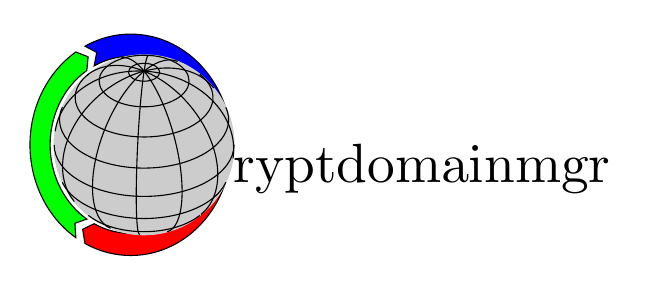
\begin{tikzpicture}
  \begin{scope}[x=9.1,y=10]
  \foreach \x\c in \elems {
	  \arcarrow{3.2}{3.6}{4}{360/\n*(\x-0.5)+\gap+\offset}{360/\n*(\x+0.5)-\gap+\offset}{5}{\c, draw = black}{}%
  }
  \end{scope}
  \begin{scope}[shift={(0.17,0)},rotate=0,x=10,y=10]
  	\def\R{3.25} % sphere radius
  	\def\angEl{35} % elevation angle
  	\filldraw[ color=black!20!] (0,0) circle (\R);
  	\foreach \t in {-80,-60,...,80} { \DrawLatitudeCircle[\R]{\t} }
  	\foreach \t in {-5,-35,...,-175} { \DrawLongitudeCircle[\R]{\t} }
  \end{scope}
  \begin{scope}[shift={(3.7,-0.3)},scale=2, every node/.append style={transform shape}]
    \node at (0,0) {ryptdomainmgr};
  \end{scope}
 \end{tikzpicture}
 
\end{document}
